\problemname{Sort the Playlist}
You have a playlist with $N$ songs of different lengths in a given order. You want to sort the list so that the shortest
songs come first and the longest songs come last.

What is the minimum number of swaps you need to make to get the list sorted?
In a swap, you choose two adjacent songs and swap their positions.

\begin{figure}[ht!]
\centering
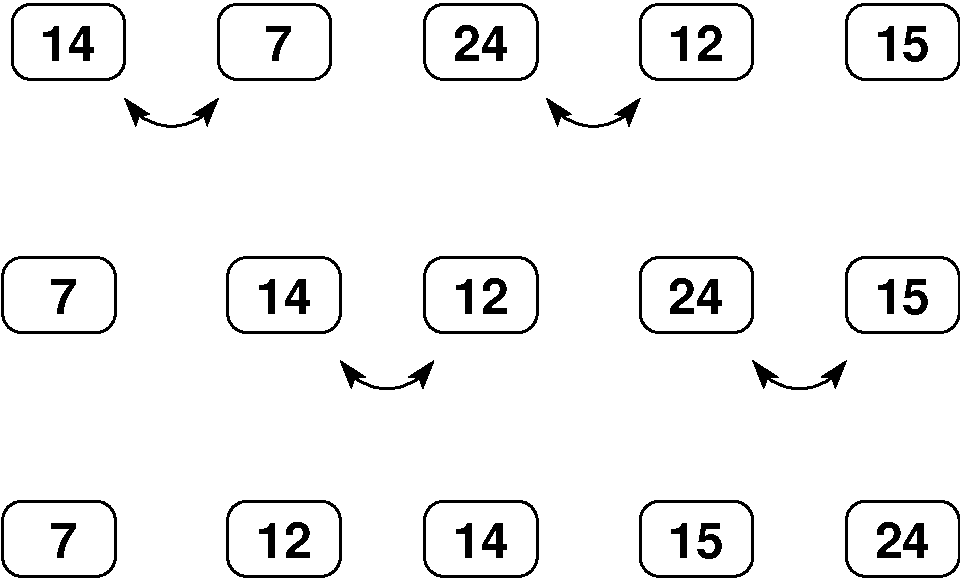
\includegraphics[width=5cm]{sorterafig.pdf}
\caption{The top row shows the starting order of the songs in the first example. The arrows show the swaps needed to sort the playlist (bottom row)}
\end{figure}

\section*{Input}
The first line of input contains an integer $N$, ($1 \leq N \leq 1000$), the number of songs.

Then follow $N$ lines. Each line contains an integer $l$ ($1 \leq l \leq 1000)$, the length of each song.
All songs have different lengths.

\section*{Output}
Output a single number: the minimum number of swaps needed to sort the playlist.

\section*{Scoring}
Your solution will be tested on a set of test groups.
To earn points for a group, you must pass all test cases in that group.

\noindent
\begin{tabular}{| l | l | p{12cm} |}
  \hline
  \textbf{Group} & \textbf{Points} & \textbf{Constraints} \\ \hline
  $1$    & $60$        & $N \leq 100$ \\ \hline 
  $2$    & $40$        & No additional constraints. \\ \hline 
\end{tabular}
